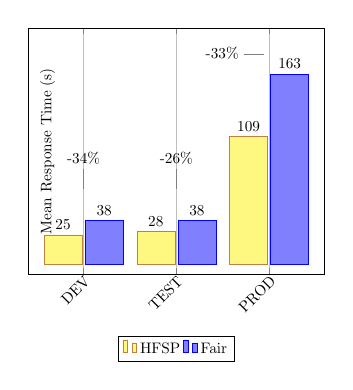
\begin{tikzpicture}[scale=0.55]
  \begin{axis}[
    ybar,
    bar width=25pt,
    ymin=31,
    enlarge y limits={upper,value=0.15},
    legend style={at={(0.5,-0.25)},
    anchor=north,legend columns=-1},
    ylabel={Mean Response Time (s)},
    ylabel style={yshift=-0.75cm},
    symbolic x coords={DEV, TEST, PROD},
    xtick=data,
    xticklabel style={
        inner sep=0pt,
        anchor=north east,
        rotate=45
    },
    xtick align=inside,
    ytick=\empty,
    nodes near coords={\pgfmathprintnumber[fixed,precision=0]{\pgfplotspointmeta}},
    enlargelimits=0.30,
    grid = major,
    ]
    \addplot[fill=yellow!50!white,draw=brown] coordinates {(DEV,25.3) (TEST,28.3) (PROD,109.3)};
    \addplot[fill=blue!50!white,draw=blue] coordinates {(DEV,37.5) (TEST,37.5 ) (PROD,162.5)};
    \legend{HFSP,Fair}

    \node[pin=above:-34\%] at (axis cs:DEV,60) {};
    \node[pin=above:-26\%] at (axis cs:TEST,60) {};
    \node[pin=left:-33\%] at (axis cs:PROD,180) {};

  \end{axis}
\end{tikzpicture}

